\section{Cells as functions}
\label{introduction:hierarchy}

Abstracting cell biological systems into mathematical or computational
models can be a powerful way to learn about those systems, though the
value of any given model can vary tremendously. If a model is as
complicated as the system it represents,
we have learned nothing; if the model is too simple, we have not captured
the biology we are trying to understand. In any case, the process of modeling
itself brings a rigor to and an awareness of the studied system that might not have
otherwise been possible \cite{Janes2013,Zhang2013,Pe'er2011}.


This section is primarily intended for classically trained
biologists, like myself, who are not often exposed to this way of thinking.
Those in fields that are historically more modeling-oriented,
such as computer science and systems biology, will likely find the following
to be familiar.


\subsubsection{Setting up an abstraction}


A useful abstraction when developing models of
cell signaling is to think of cells
as functions $f$ that convert sensory inputs $S$
into behavioral responses $R$, such that $f(S)=R$. For example,
$S$ may be the concentration of an extracellular ligand, while
$R$ may be the nuclear concentration of a downstream
transcription factor, so that $f(S)$ models the
behavior of a receptor that converts one to the other.
The function, then, is typically the biological process that we wish
to understand.


I borrow the term ``encoding'' from computer science
to refer to this relationship, because it carries with it the
idea that it is \b{information} that is being converted from one form to another.
Using this language,
$f$ encodes $S$ into $R$. Take human speech as an example. 
In speech our brains generate
words that are encoded into complex temporal patterns of
vocal chord tension, lung contraction, tongue movement, and so
on. Those patterns in turn encode temporal changes in air
pressure that propagate away from the speaker. Cells
in the ear of the listener encode those pressure changes into
mechanical movements, which then encode those movements into
neuronal activity that the listener finally decodes into the
original spoken words.


For experiments in this framework, $S$ is whatever
experimental perturbation is being applied, $R$ is the
experimental readout, and $f$ is the biological encoding process that
we are trying to understand. The assumption in our experiments,
then, is that knowledge of $S$ and $R$ are sufficient to infer
$f$. When we first dive into the complete unknowns of a
phenomenon, a precise inference is essentially impossible.
As a consequence, we find ourselves using vague
words to describe $f$, such as ``recruits,'' ``activates,''
or ``mediates''; the function remains a mystery.


For values of $S$ and $R$ that are
closely connected by some process, experiments allow us
to associate more precise
mechanisms with $f$, so that we can describe the function with words like ``binds''
or ``phosphorylates.'' However, for values of $S$ and $R$
that are distantly connected, perhaps through other nodes such as in the 
case of speech described above,
clear definitions of $f$ become more difficult. This
is a constant struggle in the study of developmental signaling pathways,
as studied in this dissertation, because many of their
interesting biological effects are far removed in time from the
signaling event. Activation of these pathways may therefore
induce many complex layers of signal processing before finally affecting $R$
\arp{fig:introduction:function}: the function is a composition of functions.


To precisely model mechanism in such cases, collapsing the
relationship between $S$ and $R$ into an understandable function is impossible.
Instead we would need to break the original function into many, where
the output of each function becomes the input for the next
(\ar{fig:introduction:function}), and study them individually.
By breaking up a general, indirect model (e.g. ``Wnt blocks
stem cell differentiation'') into a set of more specific models with direct
relationships (e.g. ``Wnt binds Frizzled, resulting in
increased \bcat, which in turn binds to the Myc promoter and
increases its expression''), we obtain insight about mechanistic details
at the cost of simplicity.


  \begin{figure}[!bt]
  \centering
  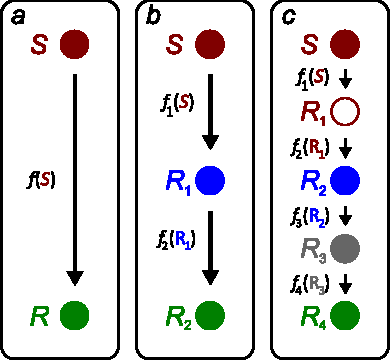
\includegraphics[width=2.5in]{FIGS/introduction/function.pdf}
  {\singlespacing 
  \caption[Abstracting signaling as a hierarchy of functions.]
          { Cells can be abstracted as functions that take sensory
			inputs $S$ and yield output responses $R$. However, interpretation of this
			abstraction suffers from unknowns between the initial
			input $S$ and the final output of interest $R$ (\b{a}). By adding
			more (\b{b}) and more (\b{c}) components the model becomes
			complex but each link gains functional insight.}
  \label{fig:introduction:function}}
  \end{figure}


  
As an additional point, for a given biological function $f$ there can be
multiple inputs and outputs, many (or most) of which are unknown.
And so the inputs and outputs are better thought of
as lists or vectors, as in equations
\ref{eq:introduction:inputs}-\ref{eq:introduction:function}
(bold face, non-italics indicate a vector).
In this model, the true
values of $\vec{S}$ are the known and experimental parameters
as well as any unmeasured parameters
(e.g. $S_1$ to $S_3$ may represent treatment duration,
treatment concentration, and ambient temperature). The values
of $\vec{R}$ are the measured responses as well as any unmeasured
cellular parameters that change in response to $\vec{S}$.
To complicate
matters, each parameter may have completely different units
(e.g. concentration versus temperature).
We must inevitably approximate the true
biological parameter vectors $\vec{S}$ and $\vec{R}$
by choosing a small known subset of their values, and
thus can only ever obtain estimates of the true function $f$.
%
    \begin{gather} 
    \vec{S}  = [S_1\cdots S_n] \label{eq:introduction:inputs} \\
    \vec{R}  = [R_1\cdots R_m] \label{eq:introduction:outputs} \\
    f(\vec{S})  =\vec{R} \label{eq:introduction:function}
    \end{gather}


Aside from the obvious issue that our approximate
models can only include things that we know about, cellular functions are often highly
non-linear. That is, it need not be true that $f(S_{1a}+S_{1b})=f(S_{1a})+f(S_{1b})$,
where $S_{1a}$ and $S_{1b}$ are different values for the same parameter,
nor that $f(aS)=af(S)$, where $a$ is a constant. A typical dose-response
curve makes a good example, since doubling the dose
(by setting $a=2$) does not necessarily double the output (i.e. $f(2S)\neq 2f(S)$).
Temporal feedback makes the models even more complex, since this 
allows a function to eventually modify its own input.
	

\subsubsection{Making use of the abstraction}


To summarize, we can think of cells as
hierarchies of functions, where the true signals $\vec{S}$ and responses $\vec{R}$
make up the nodes
of a signaling network, and the functions are the mechanistic activities that
connect them in time. The functions we study may take into account
many parameters of which we are completely unaware, and so we only obtain
estimates of $f$. Our goal in studying cell signaling is to estimate $f$
as accurately as possible, so that $f(S)\approx f(\vec{S})$.
Finally, to be able to assign a clear functional meaning to
a particular $f(S)=R$ relationship,
$S$ and $R$ must be closely connected.


A common approach to modeling signaling pathways,
that allows for both non-linearity and temporal feedback, is to assemble systems
of ordinary differential equations for
every known node and edge in the network and to explore the behavior
of the system computationally. Even a small non-linear network
can generate a wide variety of outcomes given different parameters
or small changes in topology
\cite{Shoval2010a,Wang2013b,Goentoro2009,Kholodenko2006}. Therefore, we can test
the completeness of our understanding of a signaling pathway by, for example,
testing the robustness of the model's output
against a wide array of biologically reasonable parameters (analogous to experimental
perturbations). Such approaches can
uncover deficiencies in our knowledge, as the fragility or
failures of the model may indicate a missing function or node.
Unfortunately, it is not true that successful recapitulation of a biological behavior by a
mathematical or computational model implies that we have captured
the true biology with that model.


Given the potential complexity of biological signaling models, and
the high likelihood that any given model is incomplete or flat-out
wrong, what is the value in developing models at all? I have already noted
that models give us the
potential to identify deficiencies in our knowledge, and
that building models forces us to rigorously define the questions
we seek to address. There is an additional important benefit, which is
that models may allow us to uncover underlying simplicity.


If a model
is built that recapitulates a biological phenomenon, then parts of
the model can be removed in order to determine the minimal set of
components that could create the observed biological behaviors. Having identified
these nodes one can convert a complex mechanistic model into a simple conceptual one
\cite{Ku2012,Dutkowski2011}. Additionally, if a behavior can be represented by
a highly simplified version of the functions that cause it, we can begin to
ask why the system is more complicated than it needs to be. We must be
careful with such ``why'' questions, since biological functions are created
via a random evolutionary process. However, such questions can
lead to biological insights about benefits to regulation or signal processing
of the more complex observed signaling network.

  

